\chapter{Final Architecture}
\label{ch:finarch}

\vspace{-1cm}
\begin{center}
Paolo Dini, Giuseppe Littera, Eduard Hirsch and Luca Carboni
\end{center}

\section{Introduction}


\begin{figure}[h]
\centering
\frame{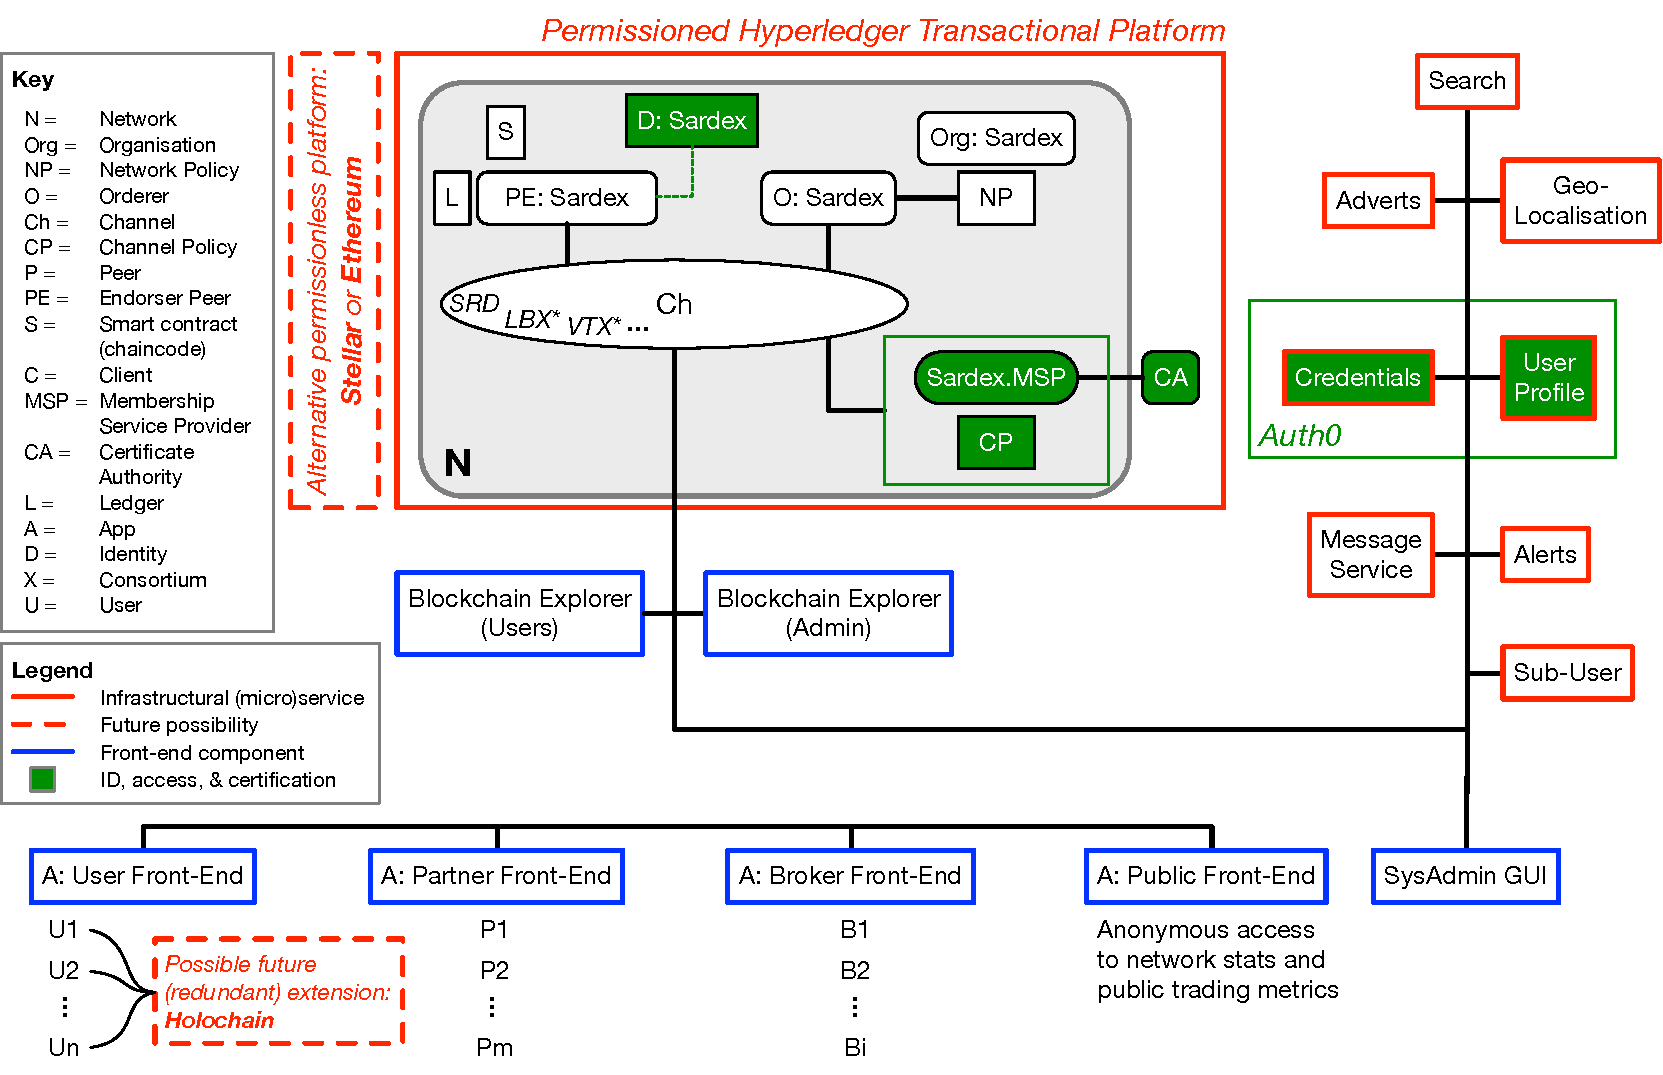
\includegraphics[width=16 cm]{Figures/HL_Architecture}}
\caption{\bf \small High-level Hyperledger-based microservice architecture with possible extensions}
\label{fig:HL_Architecture}
\end{figure}








\subsection{cto-model}
\label{sec:cto-model}



The CTO-model is specific to hyperledger composer framework and offers a possibility to set-up a ground model which is imposed onto the chain-code implementation as well as on the block-chain residing on the peers. 

The model created for Interlace project has 2 main \textit{transactions}, that are \textit{CreditTransfer} and \textit{DebitTransfer} and inherited by \textit{Transfer}. \textit{DebitTansfer} actually also needs a second transaction named \textit{DebitTransferAcknowledge} to be performed, thus it may be counted as a main transaction as well. Two other transactions supporting the functionality of the network are \textit{InitBlockchain} and \textit{CleanupPendingTransfer}.

Transfers are handling \textit{assets}, which means creating and updating them. When the main transfers are executed they are changing \textit{Account}-assets, namely, \textit{SysAccount} and \textit{MemberAccount} which are inheriting from it. \textit{DebitTransfer} also needs \textit{PendingTransfer}-asset for creating transfers which haven't yet been confirmed. \textit{DeltaDebt} collects all transfers with the negative amount portion to log when the debt has to be paid back.


\begin{figure}[h]
\centering
\frame{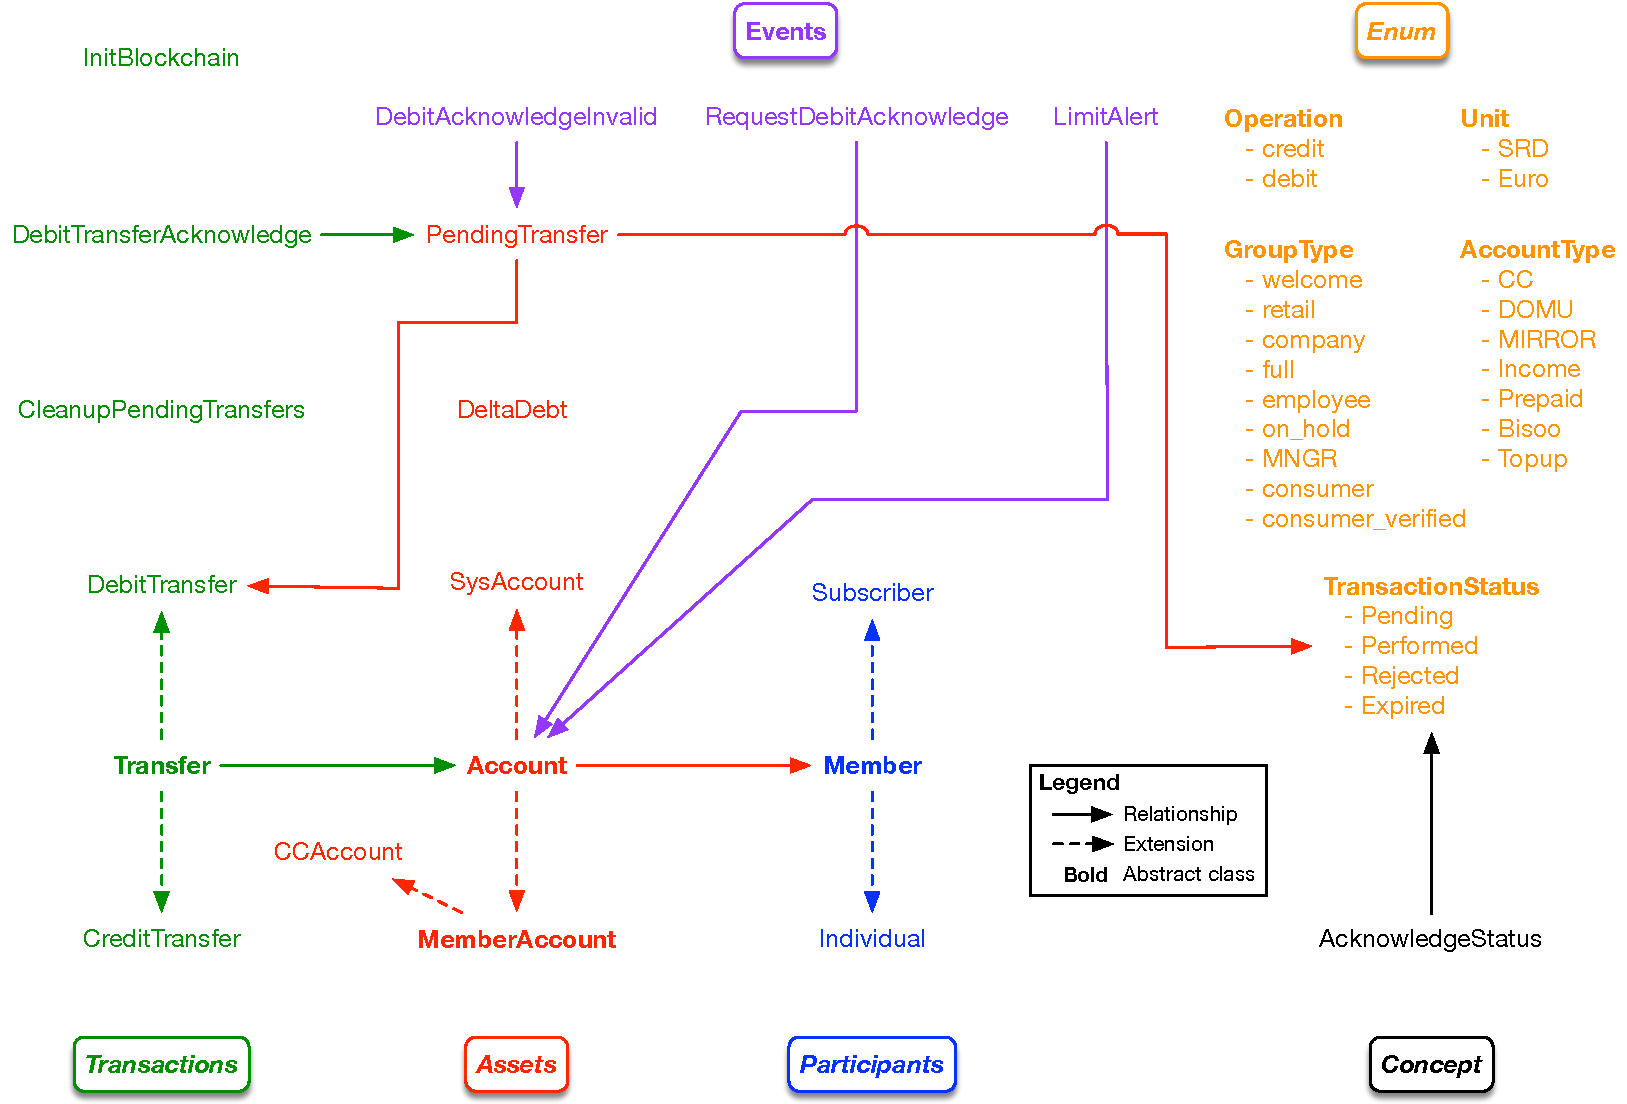
\includegraphics[width=16 cm]{Figures/DCN}}
\caption{\bf \small Hyperledger .cto model/class diagram of INTERLACE transactional platform}
\label{fig:DCN-cto}
\end{figure}

In order to perform credit or debit operations a \textit{participant} need to be registered. For the prototype they are quite reduced like the assets, however, there two participants derived from \textit{Member} called \textit{Subscriber} and \textit{Individual}. Those members may own an account asset which can be used then to transfer money from one account to another one.

On several occasions event are emitted which may be consumed by an application or a user to react to specific issues happened during a transaction. There are many different events interesting for a user but for the moment there are three implemented. One is for a forecast of a possible limit violation named \textit{LimitViolation}, \textit{RequestDebitAcknowledge} asks a user to give an acknowledgement to a pending transaction and last \textit{DebitAcknowledgeInvalid} informs that the acknowledgement for a pending transaction got denied or has been invalid.

Finally there are couple of \textit{enum} types giving states names like for operations and units as well as account and group types.

A detailed explanation of the model language can be found the official hyperledger composer documentation\footnote{\url{https://hyperledger.github.io/composer/latest/reference/cto_language.html}}



































\newpage











